\chapter{Gain in function of the frequency}
In a real op-amp the open loop gain ($A_{ol}$) is a function of the input frequency. In this experience we explored systematically this behaviour using 2 different circuits, one for the lower frequencies and the other for the higher ones. After this study we built a non inverting amplifier with $\approx 10$ and $\approx 100$ gain for measuring its bandwidth.

\section{Materials}
\begin{itemize}
\item Operational amplifier uA741
\item Resistors, trimmers, capacitors
\item Power supply RIGOL DP831A
\item Waveform generator RIGOL DG1032
\item Multimeter RIGOL DM3068
\item Oscilloscope RIGOL MS02102A
\end{itemize}
The resistor chosen were $R_1, R_2, R_3 = 10\text{k} \Omega$, $R_4 = 10 \Omega$, $R_5 = 100 \Omega, R_6 = 1\text{k}\Omega$ with an error of $5\%$ of the value.

\section{Experimental setup}
\begin{figure}[H]
\centering
\begin{minipage}{.5\textwidth}
  \centering
\begin{circuitikz}
\draw(0,0) node[op amp] (opamp) {}
	%(opamp.+) node[left] {$v_+$}
	(opamp.+) to[short] (-1.5,-.49)to[short](-1.5,-1.5)to[short](-2.5,-1.5)
	(opamp.out) to [short,-o](1.8,0) node[right] {$v_o$}
	(opamp.down) ++(0,-.5) node[below] {$-v_{cc}$} -- (opamp.down)
	(opamp.up) ++ (0,.5) node[above] {$+v_{cc}$} -- (opamp.up)
	(opamp.down) ++ (0,-.25)to[C,/tikz/circuitikz/bipoles/length=1cm] (1,-.8)node[ground,rotate = 90,yshift = 1em] {}
	(opamp.up) ++ (0,.25)to[C,/tikz/circuitikz/bipoles/length=1cm] (1,.8)node[ground,rotate = 90,yshift = 1em] {};
	\draw(opamp.-) to[short](-2.5,.49) to[R=$R_3$,-*](-2.5,2.2)node[above]{$v_a$} to[R,l=$R_2$](1.5,2.2) to[short](1.5,0);
	\draw(-2.5,.49)to[R,l_=$R_4$](-2.5,-1.5) node[ground]{};
	\draw(-4.5,.49)node[ground]{}to[sV](-4.5,2.2) to[R = $R_1$](-2.5,2.2);
\end{circuitikz}
\caption{$A_{ol}$ measure low frequencies}
\end{minipage}%
\begin{minipage}{.5\textwidth}
\begin{circuitikz}
\draw(0,0) node[op amp] (opamp) {}
	%(opamp.+) node[left] {$v_+$}
	(opamp.+) ++ (-.3,0) node[ground] {} -- (opamp.+) 
	(opamp.out) to [short,-o](1.8,0) node[right] {$v_o$}
	(opamp.down) ++(0,-.5) node[below] {$-v_{cc}$} -- (opamp.down)
	(opamp.up) ++ (0,.5) node[above] {$+v_{cc}$} -- (opamp.up)
	(opamp.down) ++ (0,-.25)to[C,/tikz/circuitikz/bipoles/length=1cm] (1,-.8)node[ground,rotate = 90,yshift = 1em] {}
	(opamp.up) ++ (0,.25)to[C,/tikz/circuitikz/bipoles/length=1cm] (1,.8)node[ground,rotate = 90,yshift = 1em] {};
	\draw(opamp.-) to[short](-2.5,.49) to[short,-*](-2.5,2.2)node[above]{$v_a$} to[R,l=$R_2$](1.5,2.2) to[short](1.5,0);
	\draw(-4.5,.49)node[ground]{}to[sV](-4.5,2.2) to[R,l=$R_1$](-2.5,2.2);
\end{circuitikz}
\caption{$A_{ol}$ measure high frequencies}
\end{minipage}
\end{figure}
In this experience we took the measurament in all circuits by changing the frequency of the input, that was a  sine wave signal 1 V peak-peak. The voltage chosen is not important, because we are interested in the ratio between the amplitude of the output and the input signals.\\
The first circuit was used for calculating the gain in the open loop configuration ($A_{ol}$) at low frequencies by measuring $v_a$ and $v_{o}$. This circuit was chosen for low freqencies instead of the second one, because the gain is too high for us to acquire directly the voltage difference between the two input pins. 
We didn't measure at frequencies lower than 30 Hz because the noise didn't allow us to make a reliable estimate of the two signals amplitude.\\
In the second circuit we measured $v_{o}$ and	 the voltage of the non inverting pin $v_a$. The frequencies measured went from 10 kHz to 200 kHz, because with high frequencies the absolute value of $A_{ol}$ is low enough.\\
In the last two circuits we built a non inverting amplifier (with a compensated offset) with a closed loop gain of 100 and 10, in order to verify the passing bandwidth.
\begin{figure}[H]
  \centering
  \begin{circuitikz}
 \draw(0,0) node[op amp,yscale=-1] (opamp) {}
%(opamp.+) node[left] {$v_+$}
(opamp.-) ++ (-.3,0) -- (opamp.-) 
(opamp.-) ++ (-.3,0) to[R,l_=$R_4$] (-3,-0.5) to (-3,-1) node[ground]{}
(opamp.-) ++ (-.3,0) -- (-1.5,-1.8) to[R,l_=$R_5$] (1,-1.8) -- (1,0)
(opamp.out) node[right] {$v_o$}
(opamp.up) ++(0,-.5) node[below] {$-v_{cc}$} -- (opamp.up)
(opamp.down) ++ (0,.5) node[above] {$+v_{cc}$} -- (opamp.down);
\draw(-4,-1) to[sV,l=$v_{in}$] (-4,.5) to[short] (opamp.+);
\draw(-4,-1) node[ground] {};
\end{circuitikz}
\caption{Non inverting amplifier}
\end{figure}

\section{Data Analysis}
\begin{figure}[H]
\centering
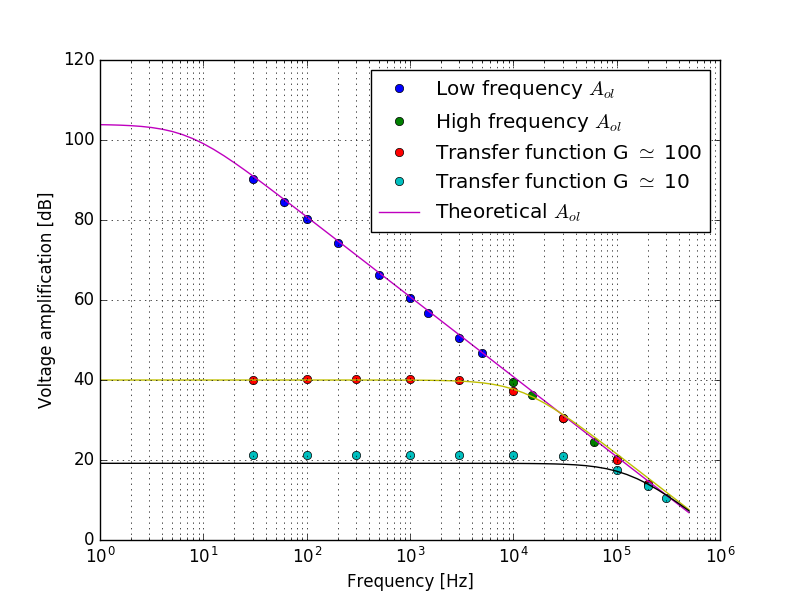
\includegraphics[width=.7\textwidth]{4/decibel.png}
\caption{Gain as a function of the frequency}
\end{figure}
Using the first circuit we can estimate from the formula $A_{ol} = - \frac{v_{o}}{v_a} \frac{R_3 + R_4}{R_4}$.
The same can be done with the second circuit, but this time the formula comes to be $A_{ol} = - \frac{v_{o}}{v_a}$. \\
We can see from the plot that the data appears to be on a straight line and it is also visible that this line is compatible with the values in the datasheet (the continuous line).
We can  however compute the theoretical open loop gain with: $$A_{ol}^{teo}(f) = \frac{A}{1 + j\frac{f}{f_0}}$$ where $f_0 = 8$ Hz is a parameter available in the datasheet and  $A = 1.5 \times 10^5$ was obtained with the best fit, $j$ is the immaginary unit and $f$ is the frequency. We can see from the plot that our data is consistent with the theory and the datasheet.\\
Regarding the last two circuit we plotted $H = \frac{v_{o}}{v_{in}}$ (the dots in the graph, experimental values), while the theoretical curve has been obtained thanks to the following formula:
\[H(f) = \frac{\frac{A}{1 + A \beta}}{1 + j \frac{f}{(1 + A \beta)f_0}}\]
where $\beta = \frac{R4}{R5+R4}$.\\
With a closed loop gain $G$ of 100 we have a cutoff frequency of nearly $10^4$ Hz, while with $G = 10$ it becomes 10 times higher, as anticipated. This means that as long as we keep low the gain of our circuit, we can use a wider range of frequencies. 
